\documentclass[a4paper,12pt]{report}

% --- Encodage et langue ---
\usepackage[utf8]{inputenc}
\usepackage[T1]{fontenc}
\usepackage[french]{babel}

% --- Mise en page ---
\usepackage[a4paper, margin=2.5cm]{geometry}
\usepackage{parskip}
\usepackage{setspace}
\linespread{1.3}
\setlength{\parindent}{0pt}

% --- Graphiques et tableaux ---
\usepackage{graphicx}
\usepackage{float}
\usepackage{array}
\usepackage{tabularx}

% --- Mathematiques et code (ajouts pour ce rapport) ---
\usepackage{amsmath}
\usepackage{amssymb}
\usepackage{listings}
\usepackage{xcolor}
\usepackage{enumitem}

% --- Liens ---
% hidelinks : sans cette option, hyperref encadre en rouge chaque entree de la
% table des matieres, ce qui alourdit fortement le rendu a l'impression.
\usepackage[hidelinks]{hyperref}

% --- En-têtes et pieds de page ---
\usepackage{fancyhdr}
\pagestyle{fancy}
\fancyhf{}
\setlength{\headheight}{50pt}

\fancyhead[L]{%
  \vspace{5pt}%
  
\includegraphics[height=1.2cm]{images/emsi.png}%
}
\fancyhead[C]{%
  \vspace{5pt}%
  \leftmark
}
\fancyfoot[C]{\thepage}

% --- Cadre esthétique ---
\usepackage{tikz}
\usepackage{atbegshi}
\AtBeginShipout{\AtBeginShipoutAddToBox{%
  \begin{tikzpicture}[remember picture,overlay]
    \draw[line width=0.5pt,gray]
      ([xshift=1cm,yshift=-1cm]current page.north west)
      rectangle
      ([xshift=-1cm,yshift=1cm]current page.south east);
  \end{tikzpicture}%
}}

% --- Pour une table des matières plus esthétique ---
\usepackage{tocloft}
\usepackage{needspace}

\setlength{\cftbeforechapskip}{10pt}
\setlength{\cftbeforesecskip}{5pt}
\setlength{\cftbeforesubsecskip}{2pt}

\setlength{\cftchapindent}{0pt}
\setlength{\cftsecindent}{10pt}
\setlength{\cftsubsecindent}{20pt}

\renewcommand{\cftchapfont}{\normalsize\bfseries}
\renewcommand{\cftsecfont}{\normalsize}
\renewcommand{\cftsubsecfont}{\small}

% --- Styles propres a ce rapport ---
\definecolor{codebg}{RGB}{246,247,249}
\definecolor{accent}{RGB}{59,110,165}
\definecolor{warn}{RGB}{192,57,43}

\lstset{
  basicstyle=\ttfamily\footnotesize,
  backgroundcolor=\color{codebg},
  breaklines=true, frame=single,
  framesep=4pt, xleftmargin=6pt, numbers=none, showstringspaces=false
}

\emergencystretch=2.5em

% --- Reglages de mise en page : eviter les pages creuses -------------------
% Le bloc de texte est allonge : avec des marges de 2,5 cm et un interligne de
% 1,3, chaque page portait peu de lignes, ce qui multipliait les fins de
% chapitre debordant de deux ou trois lignes sur une page suivante vide.


% Les flottants sont places en [htbp] ; ces parametres autorisent LaTeX a
% remplir davantage chaque page plutot qu'a ejecter une page a moitie vide.
\renewcommand{\topfraction}{0.9}        % part max de la page pour les flottants en haut
\renewcommand{\bottomfraction}{0.8}     % idem en bas
\renewcommand{\textfraction}{0.07}      % part min de texte sur une page mixte
\renewcommand{\floatpagefraction}{0.75} % remplissage min d'une page de flottants
\setcounter{topnumber}{3}
\setcounter{bottomnumber}{2}
\setcounter{totalnumber}{5}

% Evite les lignes orphelines et veuves, qui provoquent des debordements d'une
% ou deux lignes sur la page suivante.
\widowpenalty=10000
\clubpenalty=10000

% Titres de chapitre : l'espace par defaut (50pt au-dessus, 40pt en dessous)
% laisse un quart de page vide a chaque ouverture de chapitre.
\makeatletter
\renewcommand\chapter{%
  \if@openright\cleardoublepage\else\clearpage\fi
  \thispagestyle{fancy}%
  \global\@topnum\z@
  \@afterindentfalse
  \secdef\@chapter\@schapter}
\def\@makechapterhead#1{%
  \vspace*{6pt}%
  {\parindent \z@ \raggedright \normalfont
    \ifnum \c@secnumdepth >\m@ne
        \Large\bfseries \@chapapp\space \thechapter
        \par\nobreak
        \vskip 8\p@
    \fi
    \interlinepenalty\@M
    \Huge \bfseries #1\par\nobreak
    \vskip 20\p@
  }}
\def\@makeschapterhead#1{%
  \vspace*{6pt}%
  {\parindent \z@ \raggedright \normalfont
    \interlinepenalty\@M
    \Huge \bfseries #1\par\nobreak
    \vskip 20\p@
  }}
\makeatother

% =============================
% Début du document
% =============================
\begin{document}

% -------- Page de garde --------
\begin{titlepage}
    \begin{center}
        % Logos
        \begin{minipage}{0.45\textwidth}
            \centering
            
\includegraphics[width=0.4\textwidth]{images/emsi.png}
        \end{minipage}
        \hfill
        \begin{minipage}{0.45\textwidth}
            \centering
            
\includegraphics[width=0.8\textwidth]{images/honoris.png}
        \end{minipage}

        \vspace{1.5cm}

        \textsc{\LARGE EMSI : École Marocaine des Sciences de l'Ingénieur}\\[0.4cm]

        \rule{\linewidth}{0.5mm} \\[0.4cm]
        {\Huge \bfseries Reconnaissance d'émotions faciales par apprentissage profond}\\[0.3cm]
        {\Large \bfseries Conception, implémentation et validation d'un réseau de neurones convolutif sur FER2013}\\[0.4cm]
        \rule{\linewidth}{0.5mm} \\[1.8cm]

        {\Large \textit{Mini-Projet Académique}}\\[1.2cm]

        \begin{flushleft}
        \textbf{Réalisé par :} Gourari Mohamed Amine -- Jeait Amine\\[0.5cm]
        \textbf{Filière :} Informatique et Réseaux\\
        \textbf{Groupe :} 5IIR Dev1\\
        \end{flushleft}

        \vfill
        \textsc{Année universitaire : 2025 -- 2026}
    \end{center}
\end{titlepage}


\tableofcontents
\thispagestyle{empty}

\listoffigures
\listoftables
\thispagestyle{empty}
\newpage

% =========================
% Abstract
% =========================
\chapter*{Abstract}
\addcontentsline{toc}{chapter}{Abstract}

Facial expression recognition is a computer vision task that consists in
predicting an emotional category from an image of a human face. It is now a
standard benchmark for convolutional neural networks, and it raises questions
that go well beyond raw accuracy: class imbalance, label noise, and the
distinction between an \emph{apparent expression} and a \emph{felt emotion}.

This project implements a complete facial emotion recognition system: a
convolutional neural network trained from scratch on the FER2013 dataset
(35\,887 grayscale images, seven emotion classes), together with a full
inference pipeline ranging from face detection to real-time classification on a
webcam stream. Beyond the implementation itself, this report emphasises the
\emph{verification methodology}: a set of sanity checks applied to the network
before committing to a ten-hour training run. Three real defects were detected
and corrected through this process.

\textbf{Keywords:} deep learning, convolutional neural network, facial
expression recognition, FER2013, PyTorch, class imbalance, computer vision.

% =========================
% Résumé et mots-clés
% =========================
\chapter*{Résumé}
\addcontentsline{toc}{chapter}{Résumé}

La reconnaissance d'émotions faciales est une tâche de vision par ordinateur
consistant à prédire une catégorie émotionnelle à partir de l'image d'un visage.
Elle constitue aujourd'hui un cas d'étude classique des réseaux de neurones
convolutifs, et soulève des problématiques qui dépassent la seule performance
brute : déséquilibre des classes, bruit d'annotation, et distinction entre
\emph{expression apparente} et \emph{émotion ressentie}.

Ce mini-projet consiste à réaliser un système complet de reconnaissance
d'émotions faciales : un réseau de neurones convolutif entraîné de zéro sur le
jeu de données FER2013 (35\,887 images en niveaux de gris, sept classes
d'émotions), accompagné d'une chaîne d'inférence allant de la détection du
visage jusqu'à la classification en temps réel sur un flux webcam.

Au-delà de l'implémentation, ce rapport met l'accent sur la \emph{démarche de
validation} : une série de tests de sanité appliqués au réseau avant d'engager
un entraînement de dix heures. Cette méthode a permis de détecter et de corriger
trois défauts réels. Les mécanismes mis en place --- découpage stratifié,
pondération inverse des classes, lissage des étiquettes, augmentation de données
adaptée au domaine du visage --- répondent directement aux caractéristiques
mesurées du jeu de données.

\bigskip
\noindent
\textbf{Mots-clés :} apprentissage profond, réseau de neurones convolutif,
reconnaissance d'expressions faciales, FER2013, PyTorch, déséquilibre des
classes, vision par ordinateur.

% =========================
% Introduction générale
% =========================
\chapter*{Introduction générale}
\addcontentsline{toc}{chapter}{Introduction générale}

L'analyse automatique du visage humain constitue l'un des domaines
d'application les plus actifs de l'apprentissage profond. Parmi ces
applications, la reconnaissance des expressions faciales occupe une place
particulière : elle intervient dans l'interaction homme-machine, l'assistance
aux personnes, l'analyse de l'attention ou encore la recherche en psychologie
expérimentale.

Le présent mini-projet a pour objectif de concevoir, implémenter et valider un
système complet de reconnaissance d'émotions faciales. La tâche consiste à
classer une image de visage parmi sept catégories issues du modèle des émotions
de base d'Ekman : colère, dégoût, peur, joie, neutre, tristesse et surprise.

Il convient de préciser d'emblée une nuance qui conditionne l'interprétation de
l'ensemble des résultats présentés : le système prédit une \textbf{expression
apparente}, et non une émotion réellement ressentie. Ces deux notions ne
coïncident pas, et le chapitre~\ref{chap:limites} revient en détail sur cette
limite ainsi que sur les usages qu'elle exclut.

Le travail a été structuré autour d'un principe directeur : \emph{valider avant
d'entraîner}. Un entraînement complet sur le jeu de données FER2013 demandant
environ dix heures de calcul sur processeur, engager ce temps sur une
implémentation non vérifiée reviendrait à risquer de découvrir, au bout de dix
heures, qu'un modèle n'apprenait rien --- sans savoir pourquoi. L'ensemble de la
chaîne a donc été testée au préalable sur un jeu synthétique, et le réseau
soumis à une batterie de tests de sanité indépendants des données.

Ce rapport s'articule autour de sept chapitres. Le premier présente
l'environnement de travail. Le deuxième décrit le jeu de données FER2013 et ses
statistiques. Le troisième détaille l'architecture du réseau de neurones et la
justification de chaque choix structurel. Le quatrième expose le protocole
d'entraînement. Le cinquième est consacré à la validation de l'implémentation.
Le sixième présente la chaîne d'inférence et les résultats. Le septième traite
des limites et de l'usage responsable du système.

% =========================
% Chapitre 1
% =========================
\chapter{Présentation de l'environnement de travail}

\section*{Introduction du chapitre}
La réussite d'un projet d'apprentissage profond repose en grande partie sur le
choix de l'environnement logiciel et sur la prise en compte des contraintes
matérielles. Ces contraintes ne sont pas de simples détails d'intendance : elles
déterminent directement la taille du réseau, la résolution des images et la
durée des expérimentations.

Ce chapitre présente l'environnement technique utilisé, les bibliothèques
retenues et l'organisation du code produit.

\section{Technologies utilisées}
\label{sec:technos}

L'ensemble du projet repose sur l'écosystème scientifique de Python. La
figure~\ref{fig:pile} en présente l'organisation en couches : chaque niveau ne
s'appuie que sur ceux situés en dessous de lui, ce qui permet de remplacer un
composant sans toucher au reste.

\begin{figure}[htbp]
\centering
\begin{tikzpicture}[font=\small\sffamily,
  bloc/.style    = {draw=black!55, rounded corners=3pt, minimum height=1.05cm,
                    align=center, inner sep=4pt},
  couche/.style  = {bloc, text width=12.2cm, fill=#1},
  brique/.style  = {bloc, text width=3.75cm, fill=#1}]

\node[couche=black!6] (app) at (0,0)
  {\textbf{Modules du projet}\\[1pt]
   \texttt{train} \textperiodcentered{} \texttt{evaluate} \textperiodcentered{}
   \texttt{predict} \textperiodcentered{} \texttt{realtime}};

\node[brique=blue!12]   (torch) at (-4.25,-1.75) {\textbf{PyTorch} 2.15\\réseau, gradients};
\node[brique=blue!12]   (tv)    at ( 0,    -1.75) {\textbf{TorchVision} 0.29\\images, augmentation};
\node[brique=teal!14]   (cv)    at ( 4.25,-1.75) {\textbf{OpenCV} 5.1\\visage, webcam};

\node[brique=orange!16] (sk)    at (-4.25,-3.5)  {\textbf{scikit-learn} 1.9\\métriques};
\node[brique=orange!16] (np)    at ( 0,    -3.5)  {\textbf{NumPy}\\tableaux};
\node[brique=orange!16] (mpl)   at ( 4.25,-3.5)  {\textbf{Matplotlib} 3.10\\figures};

\node[couche=black!6]  (py) at (0,-5.25) {\textbf{Python} 3.13.9};
\node[couche=black!16] (hw) at (0,-6.85)
  {\textbf{Matériel} : processeur 20 c\oe{}urs, 12 fils de calcul\\[1pt]
   accélérateur graphique présent mais inexploitable (§\ref{sec:materiel})};

\draw[->,black!45] (hw.north) -- (py.south);
\draw[->,black!45] (py.north) -- (np.south);
\draw[->,black!45] (np.north) -- (tv.south);
\draw[->,black!45] (tv.north) -- (app.south);
\end{tikzpicture}
\caption{Pile technologique du projet. Les couches basses sont imposées par la
machine, les couches hautes sont le code produit pour ce travail.}
\label{fig:pile}
\end{figure}

Le tableau~\ref{tab:technos} détaille le rôle exact de chaque composant. Les
versions sont indiquées parce qu'elles ne sont pas interchangeables : la
section~\ref{sec:diff:opencv} montre qu'un changement de version majeure
d'OpenCV a supprimé une fonctionnalité utilisée par le projet.

\begin{table}[htbp]
\centering
\caption{Technologies utilisées et rôle dans le projet}
\label{tab:technos}
\begin{tabularx}{\textwidth}{|l|l|>{\raggedright\arraybackslash}X|}
\hline
\textbf{Composant} & \textbf{Version} & \textbf{Rôle} \\
\hline
Python & 3.13.9 & Langage de développement \\
PyTorch & 2.15.0 (CPU) & Définition du réseau, calcul des gradients, optimisation \\
TorchVision & 0.29.2 & Lecture des images, augmentation, architectures pré-entraînées \\
OpenCV & 5.1.0 & Détection de visage, capture vidéo, affichage temps réel \\
scikit-learn & 1.9.1 & Métriques par classe, matrice de confusion \\
NumPy & 2.x & Calcul sur tableaux, pondération des classes \\
Matplotlib & 3.10 & Génération de toutes les figures du rapport \\
\hline
YuNet & 2023mar & Modèle de détection de visage au format \textsc{onnx} \\
FER2013 & -- & Jeu de données, 35\,887 images étiquetées \\
\hline
\LaTeX{} (MiKTeX) & 25.12 & Composition de ce rapport \\
pypdf & 6.x & Mesure automatique du remplissage des pages \\
Windows & 11 Pro & Système hôte \\
\hline
\end{tabularx}
\end{table}

\section{Contrainte matérielle et ses conséquences}
\label{sec:materiel}

La machine de développement dispose d'une carte graphique \textbf{NVIDIA
GeForce RTX 5060} de 8~Go. Elle n'a pourtant \textbf{jamais pu être utilisée},
pour une raison purement logicielle : la distribution de PyTorch installée est
la variante compilée sans \textsc{cuda}.

\begin{lstlisting}[basicstyle=\ttfamily\small,frame=single,backgroundcolor=\color{black!3}]
torch 2.15.0+cpu      <- variante sans CUDA
CUDA disponible : False
Carte detectee  : NVIDIA GeForce RTX 5060, 8 Go
\end{lstlisting}

Le suffixe \texttt{+cpu} est déterminant : cette variante ne contient
simplement pas le code capable de piloter un processeur graphique. La carte est
présente, son pilote est à jour, mais elle reste invisible pour la bibliothèque.
Passer à la variante \textsc{cuda} supposait un téléchargement de près de 3~Go
et une réinstallation complète de l'environnement, ce qui a été écarté.

Tout l'entraînement s'est donc déroulé sur processeur central. Les conséquences
sont mesurées, non estimées :

\begin{itemize}[leftmargin=*,itemsep=3pt]
  \item \textbf{Précision mixte inopérante} : ce mécanisme n'accélère les
        calculs que sur accélérateur graphique. Le code le désactive
        automatiquement sur processeur, où il ne ferait que ralentir
        l'exécution.
  \item \textbf{Résolution native conservée} : les images restent en
        $48\times48$ au lieu d'être portées à $224\times224$ comme l'exigent
        les architectures pré-entraînées courantes, ce qui aurait multiplié le
        coût par plus de vingt.
  \item \textbf{Durée prohibitive} : une époque du réseau initial demande
        \textbf{312 secondes}, soit près de cinq heures pour soixante époques.
\end{itemize}

Cette dernière conséquence s'est révélée bloquante en pratique, et non
seulement inconfortable : le premier entraînement s'est interrompu de lui-même
à la quinzième époque, après plus de deux heures de calcul, sans jamais
atteindre la convergence. C'est ce constat qui a imposé la conception d'un
réseau allégé, exposée à la section~\ref{sec:diff:leger}.

\section{Organisation du code}

Le projet a été découpé en modules à responsabilité unique, de façon à pouvoir
tester chaque maillon de la chaîne indépendamment des autres.

\begin{table}[htbp]
\centering
\caption{Organisation des fichiers du projet}
\begin{tabular}{|l|p{8.5cm}|}
\hline
\textbf{Fichier} & \textbf{Rôle} \\
\hline
\texttt{src/config.py} & Hyperparamètres, classes, chemins (source unique de vérité) \\
\texttt{src/dataset.py} & Chargement, augmentation, découpage stratifié, poids de classes \\
\texttt{src/model.py} & Réseau développé pour le projet et variantes par transfert \\
\texttt{src/train.py} & Boucle d'entraînement, ordonnancement du pas, arrêt anticipé \\
\texttt{src/evaluate.py} & Métriques par classe, matrice de confusion \\
\texttt{src/face\_detect.py} & Détection de visage (YuNet ou Haar selon la version d'OpenCV) \\
\texttt{src/predict.py} & Inférence sur image, classe réutilisable \texttt{EmotionPredictor} \\
\texttt{src/realtime.py} & Classification en temps réel sur webcam \\
\hline
\texttt{scripts/prepare\_fer2013.py} & Conversion du fichier CSV en arborescence d'images \\
\texttt{scripts/download\_face\_model.py} & Téléchargement vérifié du détecteur de visage \\
\texttt{scripts/make\_dummy\_data.py} & Jeu synthétique pour tester la chaîne sans données réelles \\
\hline
\end{tabular}
\end{table}

\needspace{10\baselineskip}
\section*{Conclusion du chapitre}
Ce chapitre a présenté l'environnement technique du projet. L'absence
d'accélérateur graphique, loin d'être un obstacle rédhibitoire, a imposé une
discipline de conception bénéfique : privilégier une architecture compacte et
bien justifiée plutôt qu'un réseau surdimensionné. L'organisation modulaire du
code constitue par ailleurs le prérequis de la démarche de validation exposée
au chapitre~\ref{chap:validation}.

% =========================
% Chapitre 2
% =========================
\chapter{Le jeu de données FER2013}

\section*{Introduction du chapitre}
En apprentissage profond, la qualité du jeu de données détermine davantage le
résultat final que le choix de l'architecture. Une analyse statistique préalable
est donc indispensable : elle révèle les difficultés spécifiques auxquelles le
modèle sera confronté et oriente les choix de conception.

Ce chapitre présente le jeu de données FER2013, sa provenance, la vérification
de son intégrité, ses statistiques descriptives et les transformations qui lui
sont appliquées.

\section{Provenance et vérification de l'intégrité}

Le jeu de données retenu est FER2013, introduit lors du concours
\emph{Challenges in Representation Learning} organisé dans le cadre de la
conférence ICML en 2013. Il est distribué sous forme d'un fichier CSV dans
lequel chaque ligne contient une étiquette, 2\,304 valeurs de pixels séparées
par des espaces, et un indicateur de partition.

L'accès à la plateforme Kaggle nécessitant un jeton d'authentification, le
fichier a été récupéré depuis un miroir public distribué sous licence MIT.
Le recours à un miroir impose cependant de vérifier que les données obtenues
correspondent bien au jeu de données de référence, et non à une variante
retraitée. Le contrôle retenu est la comparaison des effectifs :

\begin{table}[htbp]
\centering
\caption{Vérification de l'intégrité du jeu de données}
\begin{tabular}{|l|r|r|l|}
\hline
\textbf{Partition} & \textbf{Obtenu} & \textbf{Référence} & \textbf{Statut} \\
\hline
Entraînement (\texttt{Training}) & 28\,709 & 28\,709 & \textcolor{accent}{Conforme} \\
Test (\texttt{PublicTest} + \texttt{PrivateTest}) & 7\,178 & 7\,178 & \textcolor{accent}{Conforme} \\
\hline
\textbf{Total} & \textbf{35\,887} & \textbf{35\,887} & \textcolor{accent}{Conforme} \\
\hline
\end{tabular}
\end{table}

Les effectifs coïncident exactement avec la référence publiée, et aucune ligne
du fichier n'a été rejetée lors de la conversion : les 35\,887 enregistrements
ont tous été convertis sans erreur de format.

\section{Statistiques descriptives}

Trois caractéristiques du jeu de données conditionnent l'ensemble des choix
techniques décrits dans les chapitres suivants : sa taille modeste
(28\,709 images d'entraînement pour un réseau de 4{,}8 millions de paramètres),
sa très faible résolution ($48\times48$ en niveaux de gris, soit 2\,304 valeurs
par image), et surtout son fort déséquilibre entre classes.

\begin{figure}[htbp]
\centering
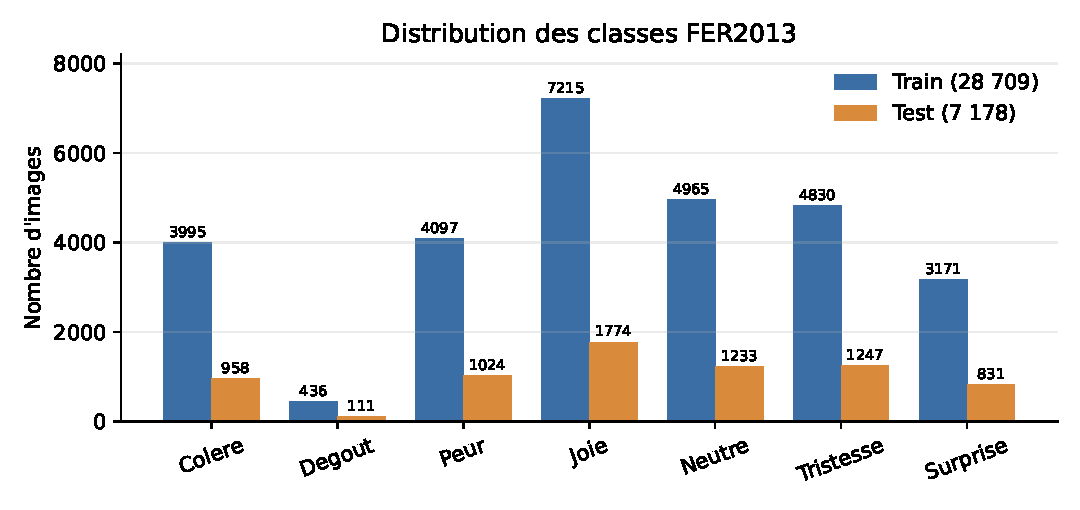
\includegraphics[width=\textwidth]{figures/distribution.pdf}
\caption{Distribution des classes du jeu de données FER2013}
\label{fig:distribution}
\end{figure}

Le déséquilibre est le trait dominant de ce jeu de données : la classe
\emph{joie} compte 7\,215 images d'entraînement contre seulement 436 pour la
classe \emph{dégoût}, soit un rapport de \textbf{16{,}5 pour 1}.

\begin{table}[htbp]
\centering
\caption{Effectifs par classe et pondération appliquée}
\begin{tabular}{|l|r|r|r|r|}
\hline
\textbf{Classe} & \textbf{Train} & \textbf{\% train} & \textbf{Test} & \textbf{Poids} \\
\hline
Joie       & 7\,215 & 25{,}1~\% & 1\,774 & 0{,}57 \\
Neutre     & 4\,965 & 17{,}3~\% & 1\,233 & 0{,}83 \\
Tristesse  & 4\,830 & 16{,}8~\% & 1\,247 & 0{,}85 \\
Peur       & 4\,097 & 14{,}3~\% & 1\,024 & 1{,}00 \\
Colère     & 3\,995 & 13{,}9~\% & 958 & 1{,}03 \\
Surprise   & 3\,171 & 11{,}0~\% & 831 & 1{,}29 \\
Dégoût     & 436 & 1{,}5~\% & 111 & \textcolor{warn}{9{,}39} \\
\hline
\textbf{Total} & \textbf{28\,709} & 100~\% & \textbf{7\,178} & \\
\hline
\end{tabular}
\end{table}

\begin{figure}[htbp]
\centering
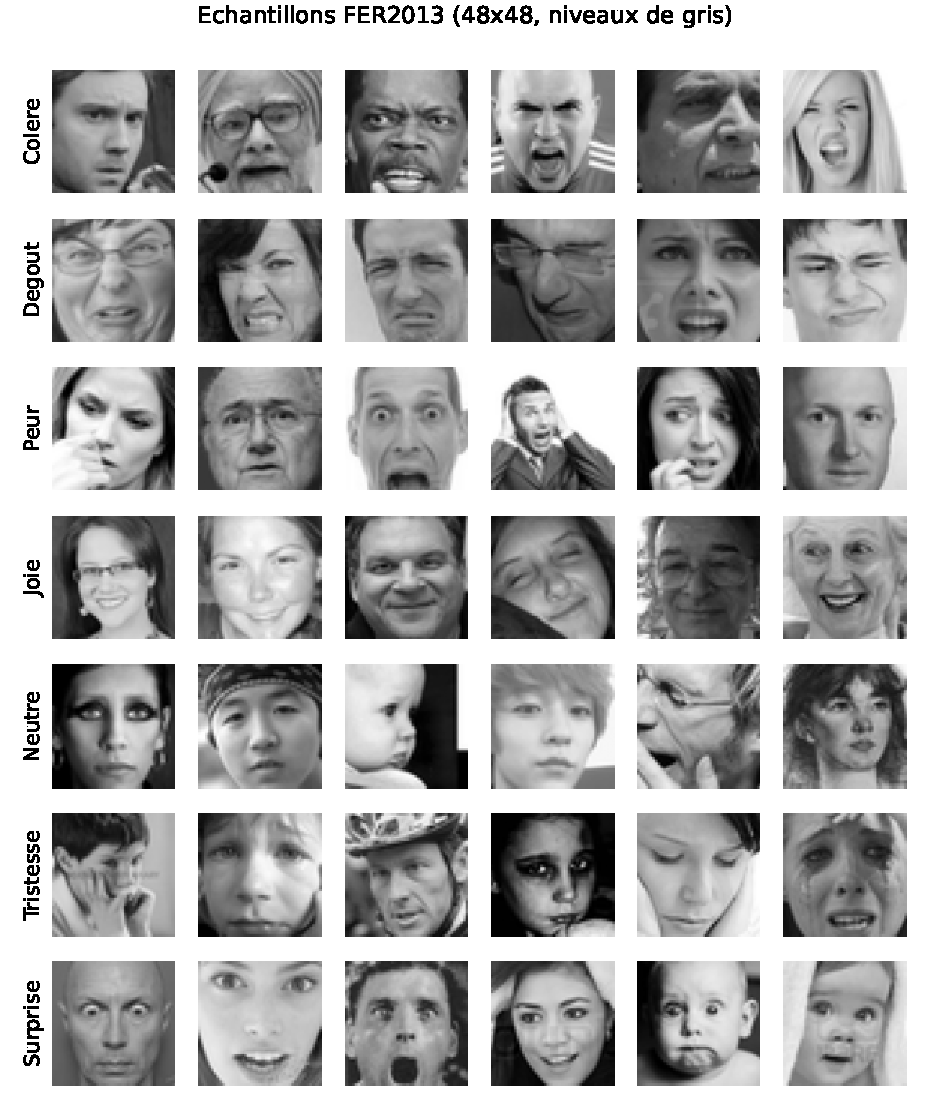
\includegraphics[width=0.78\textwidth]{figures/samples.pdf}
\caption{Échantillons réels du jeu de données, six images par classe}
\label{fig:samples}
\end{figure}

L'examen visuel de la figure~\ref{fig:samples} est instructif : les images sont
de qualité très variable, avec des poses de profil, des occlusions (mains,
lunettes), des visages d'enfants, des images floues, et même quelques étiquettes
manifestement erronées. Cette variabilité explique le plafond de performance
discuté en section~\ref{sec:plafond}.

\section{Statistiques de normalisation}

La normalisation des entrées suppose de connaître la moyenne et l'écart-type du
jeu de données. Plutôt que de reprendre des constantes trouvées dans la
littérature, ces valeurs ont été recalculées sur l'intégralité des 28\,709
images d'entraînement :

\begin{equation}
\mu = \frac{1}{N}\sum_{i=1}^{N} x_i = 0{,}5077
\qquad
\sigma = \sqrt{\frac{1}{N}\sum_{i=1}^{N} x_i^2 - \mu^2} = 0{,}2550
\end{equation}

avec $N = 28\,709 \times 48 \times 48 = 66{,}1$ millions de pixels normalisés
dans l'intervalle $[0,1]$. Le calcul emploie la forme
$\mathbb{E}[x^2] - \mathbb{E}[x]^2$ par accumulation progressive, ce qui évite
de charger 66 millions de valeurs simultanément en mémoire.

\begin{figure}[htbp]
\centering
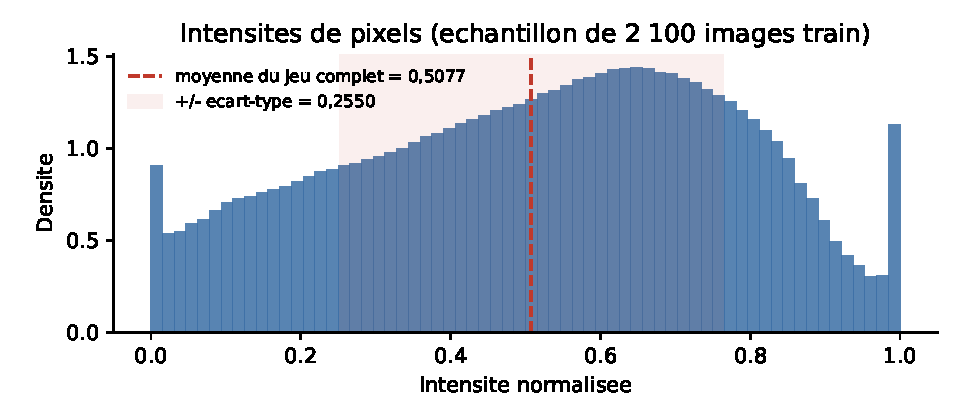
\includegraphics[width=0.74\textwidth]{figures/histogram.pdf}
\caption{Distribution des intensités de pixels du jeu d'entraînement}
\label{fig:histogram}
\end{figure}

La distribution est unimodale et légèrement asymétrique vers la gauche
(coefficient d'asymétrie $-0{,}18$, médiane 0{,}537 supérieure à la moyenne
0{,}516 de l'échantillon mesuré). Les deux pics visibles aux extrémités
correspondent à des pixels saturés : 0{,}67~\% de noir pur et 1{,}01~\% de blanc
pur, conséquence des recadrages et des surexpositions. L'étendue utile couvrant
presque toute la plage disponible, une égalisation d'histogramme supplémentaire
n'apporterait pas de contraste additionnel : la normalisation affine suffit.

Après normalisation $\hat{x} = (x - \mu)/\sigma$, les entrées du réseau sont
centrées et d'écart-type unitaire, condition nécessaire au bon fonctionnement de
l'initialisation de He décrite en section~\ref{sec:init}.

\section{Découpage entraînement, validation et test}

La partition de test (7\,178 images) est celle définie par les auteurs du jeu de
données. Elle n'est utilisée qu'une seule fois, à la toute fin, pour produire le
chiffre rapporté. La validation est extraite de la partition d'entraînement à
hauteur de 10~\%, par un \textbf{découpage stratifié} : le tirage est effectué
classe par classe.

\begin{table}[htbp]
\centering
\caption{Répartition des données}
\begin{tabular}{|l|r|p{7cm}|}
\hline
\textbf{Partition} & \textbf{Images} & \textbf{Usage} \\
\hline
Entraînement & 25\,841 & Apprentissage des poids du réseau \\
Validation & 2\,868 & Sélection du meilleur état, arrêt anticipé \\
Test & 7\,178 & Mesure finale, jamais observée pendant l'entraînement \\
\hline
\end{tabular}
\end{table}

La stratification n'est pas un raffinement théorique. Un découpage purement
aléatoire aurait pu, par malchance, placer moins de trente images de
\emph{dégoût} en validation, rendant la métrique de cette classe inexploitable
et, par conséquent, le critère d'arrêt anticipé instable.

\section{Augmentation de données}

Avec 25\,841 images d'entraînement pour 4{,}8 millions de paramètres, le
surapprentissage constitue le risque principal. L'augmentation de données est
donc appliquée de manière agressive, mais sous une contrainte forte : un visage
possède une orientation canonique.

\begin{table}[htbp]
\centering
\caption{Transformations d'augmentation et leur justification}
\begin{tabularx}{\textwidth}{|>{\raggedright\arraybackslash}X|>{\raggedright\arraybackslash}X|}
\hline
\textbf{Transformation} & \textbf{Justification} \\
\hline
Recadrage aléatoire (échelle 0{,}85--1{,}0) & Simule un cadrage imparfait du détecteur de visage \\
Symétrie horizontale ($p=0{,}5$) & Un visage en miroir reste un visage plausible \\
Transformation affine (rotation $12^\circ$, translation 8~\%, cisaillement $6^\circ$) & Inclinaison de la tête, décentrage \\
Variation de luminosité et contraste ($\pm 25$~\%) & Conditions d'éclairage variables \\
Effacement aléatoire ($p=0{,}25$) & Occlusions partielles (main, micro, mèche de cheveux) \\
\hline
\textcolor{warn}{\textbf{Pas de symétrie verticale}} & Un visage à l'envers n'existe pas dans le domaine ; cette transformation détruirait la relation spatiale \emph{yeux au-dessus de la bouche}, qui porte une grande partie de l'information d'expression \\
\hline
\end{tabularx}
\end{table}

L'ordre des opérations importe : l'effacement aléatoire s'applique
\emph{après} la normalisation, car il opère sur le tenseur et doit y insérer des
valeurs déjà à l'échelle du reste des données.

\begin{figure}[htbp]
\centering
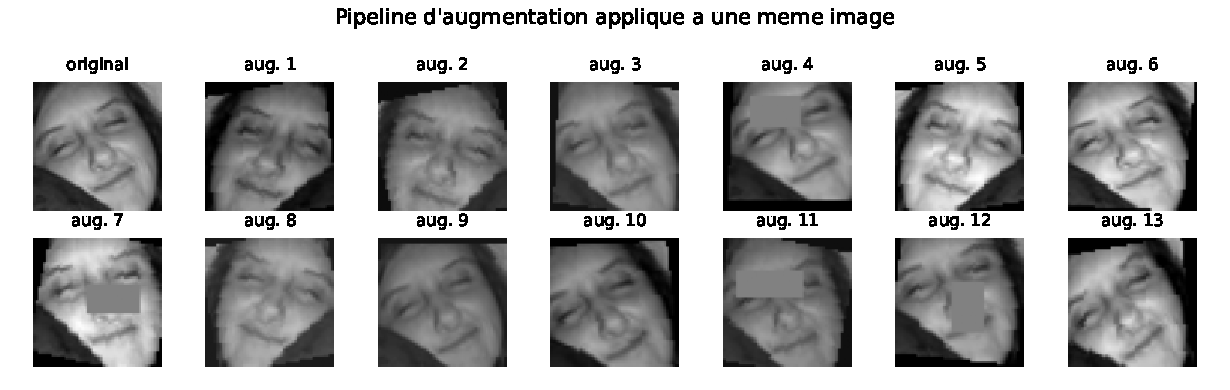
\includegraphics[width=\textwidth]{figures/augmentation.pdf}
\caption{Treize tirages successifs d'augmentation appliqués à une même image}
\label{fig:augmentation}
\end{figure}

Le réseau ne voit ainsi jamais deux fois exactement la même entrée, ce qui
l'oblige à apprendre des traits robustes plutôt qu'à mémoriser des images
particulières.

\needspace{10\baselineskip}
\section*{Conclusion du chapitre}
Ce chapitre a caractérisé le jeu de données FER2013 : son intégrité a été
vérifiée par comparaison des effectifs, ses statistiques de normalisation ont
été recalculées, et son déséquilibre de 16{,}5 pour 1 a été quantifié. Chacune
de ces mesures trouve une réponse technique directe dans les chapitres suivants :
découpage stratifié, pondération des classes et augmentation adaptée au domaine.

% =========================
% Chapitre 3
% =========================
\chapter{Architecture du réseau de neurones}

\section*{Introduction du chapitre}
L'architecture d'un réseau convolutif résulte d'un ensemble de compromis entre
capacité de représentation, nombre de paramètres et coût de calcul. Dans ce
projet, la contrainte d'un entraînement sur processeur rend ces compromis
particulièrement sensibles.

Ce chapitre décrit l'architecture retenue, justifie chacun de ses choix
structurels, et présente les variantes par transfert d'apprentissage également
implémentées.

\section{Structure générale}

L'architecture suit le schéma introduit par le réseau VGG : des blocs
convolutifs identiques empilés, chacun divisant la résolution spatiale par deux
et doublant la profondeur des cartes de caractéristiques.

\begin{table}[htbp]
\centering
\caption{Architecture détaillée du réseau}
\begin{tabular}{|l|p{5.5cm}|l|c|}
\hline
\textbf{Étage} & \textbf{Composition} & \textbf{Sortie} & \textbf{Abandon} \\
\hline
Entrée & Image en niveaux de gris & $1\times48\times48$ & --- \\
Bloc 1 & $[\text{Conv }3{\times}3 \to \text{BN} \to \text{ReLU}]\times 2 \to \text{MaxPool }2$ & $64\times24\times24$ & 0{,}20 \\
Bloc 2 & Identique & $128\times12\times12$ & 0{,}24 \\
Bloc 3 & Identique & $256\times6\times6$ & 0{,}28 \\
Bloc 4 & Identique & $512\times3\times3$ & 0{,}28 \\
Agrégation & Moyenne globale adaptative & $512\times1\times1$ & --- \\
Tête & Couche dense $512 \to 256$, BN, ReLU & $256$ & 0{,}40 \\
Sortie & Couche dense $256 \to 7$ & $7$ & --- \\
\hline
\multicolumn{3}{|l|}{\textbf{Nombre total de paramètres entraînables}} & \textbf{4\,819\,783} \\
\hline
\end{tabular}
\end{table}

Les dimensions de sortie indiquées dans ce tableau ne sont pas des valeurs
déduites sur le papier : elles ont été mesurées par propagation effective d'un
tenseur de test à travers chaque étage du réseau.

\section{Justification des choix structurels}

\subsection{Deux convolutions $3\times3$ plutôt qu'une convolution $5\times5$}

Deux couches convolutives $3\times3$ empilées couvrent le même champ réceptif
qu'une unique couche $5\times5$. Le coût en paramètres diffère toutefois
nettement : pour $C$ canaux d'entrée et de sortie, l'empilement demande
$2\times(3^2 C^2) = 18C^2$ paramètres, contre $25C^2$ pour la convolution
$5\times5$, soit une économie de 28~\%. L'empilement présente en outre
l'avantage d'intercaler une non-linéarité supplémentaire, ce qui augmente la
capacité d'expression du réseau à coût réduit.

\subsection{Normalisation par lots après chaque convolution}

La normalisation par lots stabilise la distribution des activations au fil des
couches, autorise un pas d'apprentissage plus élevé et exerce un effet de
régularisation complémentaire.

Les convolutions qui la précèdent sont déclarées sans biais. Ce point mérite
explication : le biais d'une convolution serait immédiatement annulé par
l'opération de recentrage de la normalisation qui suit. Le conserver
reviendrait à entraîner un paramètre sans aucun effet sur la sortie.

\subsection{Agrégation moyenne globale plutôt qu'aplatissement}

Ce choix est le plus déterminant de l'architecture. Un aplatissement de la carte
finale $512\times3\times3$, suivi d'une couche dense de 256 unités, coûterait
$4608 \times 256 = 1{,}18$ million de paramètres --- concentrés dans la partie du
réseau la plus sujette au surapprentissage.

L'agrégation moyenne globale réduit ce coût à $512 \times 256 = 131$ mille
paramètres, soit neuf fois moins. Elle rend par ailleurs le réseau indifférent à
la taille exacte de l'image d'entrée, ce qui facilite l'expérimentation.

\subsection{Abandon spatial croissant}

Le taux d'abandon croît avec la profondeur, de 0{,}20 à 0{,}28. Ce choix
n'est pas arbitraire : les premières couches extraient des traits génériques
(contours, textures) qu'il serait contre-productif de perturber fortement,
tandis que les couches profondes encodent des configurations spécifiques, bien
plus susceptibles d'être mémorisées.

La variante d'abandon employée désactive des canaux entiers plutôt que des
pixels isolés. C'est le comportement adapté à des activations convolutives :
les pixels voisins d'une même carte étant fortement corrélés, désactiver des
pixels isolés n'apporterait qu'une régularisation marginale.

\subsection{Initialisation de He}
\label{sec:init}

Les poids des convolutions sont initialisés selon une loi normale
$\mathcal{N}(0, \sqrt{2/n_{\text{out}}})$. Il s'agit du choix adapté aux
activations ReLU : le facteur 2 compense le fait que la fonction ReLU annule la
moitié de sa plage d'entrée, et préserve ainsi la variance du signal d'une
couche à l'autre. Le chapitre~\ref{chap:validation} vérifie expérimentalement
que cette initialisation place effectivement le réseau au point de départ
théorique attendu.

\section{Variantes par transfert d'apprentissage}

Le projet implémente également deux architectures pré-entraînées sur ImageNet :
ResNet18 (11{,}2 millions de paramètres) et EfficientNet-B0 (4{,}0 millions).

Ces réseaux attendant des images en couleurs, leur première convolution est
adaptée au niveau de gris en sommant ses poids sur la dimension des canaux de
couleur. Cette opération préserve l'information apprise, contrairement à une
réinitialisation aléatoire qui la détruirait.

Une précaution est toutefois nécessaire : ces architectures divisent la
résolution par 32. Avec une entrée $48\times48$, la carte de caractéristiques
finale se réduit à $2\times2$ et l'information spatiale est presque entièrement
détruite. Un avertissement explicite a donc été ajouté dans le script
d'entraînement lorsque la taille d'image demandée est inférieure à 64 pixels.
Cette erreur est en effet silencieuse : le code s'exécute sans incident, seule
la précision finale s'effondre.

\needspace{10\baselineskip}
\section*{Conclusion du chapitre}
Ce chapitre a présenté une architecture de 4{,}8 millions de paramètres dont
chaque composant répond à une justification précise. L'agrégation moyenne
globale et l'abandon croissant répondent au risque de surapprentissage
identifié au chapitre précédent, tandis que l'empilement de convolutions
$3\times3$ maximise la capacité d'expression sous contrainte de calcul.

% =========================
% Chapitre 4
% =========================
\chapter{Protocole d'entraînement}

\section*{Introduction du chapitre}
Le protocole d'entraînement détermine la manière dont les paramètres du réseau
sont ajustés à partir des données. Dans le cas de FER2013, il doit répondre à
une difficulté particulière déjà quantifiée : le déséquilibre considérable entre
les classes.

\section{Fonction de coût}
\label{sec:ponderation}

La fonction de coût retenue est une entropie croisée pondérée avec lissage des
étiquettes :

\begin{equation}
\mathcal{L} = -\sum_{c=1}^{7} w_c \, \tilde{y}_c \log \hat{p}_c,
\qquad
\tilde{y}_c = (1-\varepsilon)\,y_c + \frac{\varepsilon}{7},
\qquad \varepsilon = 0{,}1
\end{equation}

où $\hat{p}_c$ désigne la probabilité prédite pour la classe $c$, $y_c$
l'étiquette de référence et $w_c$ le poids attribué à la classe.

\subsection{Pondération inverse à la fréquence}

Les poids $w_c$ sont définis comme inversement proportionnels à l'effectif de
chaque classe :

\begin{equation}
w_c = \frac{N}{C \cdot n_c}
\qquad \text{avec} \quad N = 28\,709, \quad C = 7
\end{equation}

Pour la classe \emph{dégoût}, cela donne
$w = 28\,709 / (7 \times 436) = 9{,}39$, contre $0{,}57$ pour la classe
\emph{joie}.

\begin{figure}[htbp]
\centering
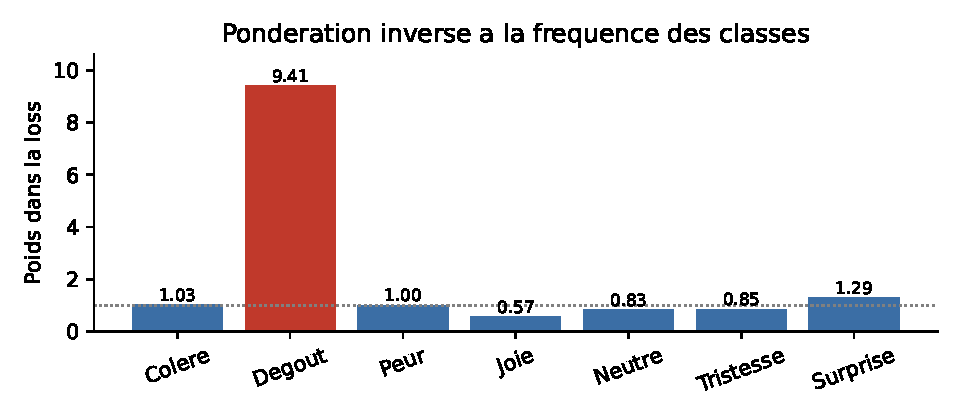
\includegraphics[width=0.74\textwidth]{figures/weights.pdf}
\caption{Pondération inverse à la fréquence appliquée à chaque classe}
\label{fig:weights}
\end{figure}

La nécessité de cette pondération se démontre simplement : un modèle qui
ignorerait complètement la classe \emph{dégoût} ne perdrait que 1{,}5~\%
d'exactitude globale. Sans pondération, l'optimiseur n'a donc aucune incitation
à apprendre cette classe.

La normalisation choisie est telle que le poids moyen, pondéré par les effectifs,
vaut exactement 1. L'échelle de la fonction de coût --- et par conséquent le pas
d'apprentissage utile --- reste ainsi comparable au cas non pondéré.

\subsection{Lissage des étiquettes}

Le lissage des étiquettes consiste à remplacer la cible binaire par une cible
légèrement adoucie. Cette technique se justifie particulièrement dans le cas
présent : les frontières entre \emph{peur} et \emph{surprise}, ou entre
\emph{tristesse} et \emph{neutre}, sont intrinsèquement floues, et les
annotations de FER2013 sont elles-mêmes bruitées. Exiger du réseau une confiance
de 100~\% sur une étiquette possiblement fausse l'encouragerait à mémoriser le
bruit d'annotation.

\section{Optimisation}

\begin{table}[htbp]
\centering
\caption{Hyperparamètres d'optimisation et leur justification}
\begin{tabular}{|l|l|p{6cm}|}
\hline
\textbf{Élément} & \textbf{Valeur} & \textbf{Justification} \\
\hline
Optimiseur & AdamW & Découple la pénalisation des poids du moment adaptatif \\
Pas initial & $10^{-3}$ & Valeur usuelle pour un réseau entraîné de zéro \\
Pénalisation & $10^{-4}$ & Régularisation $L_2$ \\
Taille des lots & 64 & Compromis entre bruit du gradient et stabilité de la normalisation \\
Montée en charge & 3 époques & Évite qu'un gradient initial mal orienté ne déstabilise les statistiques de normalisation \\
Décroissance & Cosinus jusqu'à $10^{-5}$ & Affine la convergence en fin d'entraînement \\
Écrêtage du gradient & Norme $\leq 5$ & Protège contre les lots aberrants \\
Arrêt anticipé & Patience de 12 époques & Interrompt dès que la validation stagne \\
\hline
\end{tabular}
\end{table}

\section{Sauvegarde et reproductibilité}

L'état retenu à l'issue de l'entraînement n'est pas celui de la dernière époque,
mais celui ayant obtenu la \textbf{meilleure exactitude en validation}. Les deux
états sont néanmoins conservés : l'écart entre eux renseigne directement sur
l'ampleur du surapprentissage.

Chaque sauvegarde embarque la configuration complète ayant servi à
l'entraînement : architecture, taille d'entrée, nombre de canaux et liste
ordonnée des classes. L'inférence reconstruit ainsi le modèle à partir du
fichier seul. Ce mécanisme élimine une source d'erreur classique et
particulièrement difficile à diagnostiquer : l'application, au moment de
l'inférence, d'un prétraitement incohérent avec celui de l'entraînement.

\needspace{10\baselineskip}
\section*{Conclusion du chapitre}
Le protocole d'entraînement répond point par point aux caractéristiques du jeu
de données. La pondération des classes traite le déséquilibre, le lissage des
étiquettes traite le bruit d'annotation, et la sauvegarde de la configuration
complète élimine une catégorie entière d'erreurs d'inférence.

% =========================
% Chapitre 5
% =========================
\chapter{Validation de l'implémentation}
\label{chap:validation}

\section*{Introduction du chapitre}
Ce chapitre décrit les tests appliqués au système \emph{avant} l'entraînement
long. Ces tests ne mesurent pas la qualité du modèle : ils vérifient que le code
fait effectivement ce qu'il prétend faire. Cette distinction est essentielle, et
cette étape est trop souvent omise dans les projets d'apprentissage profond.

\section{Démarche adoptée}

La démarche inverse l'ordre habituel de développement :

\begin{enumerate}[leftmargin=*,itemsep=3pt]
  \item Écrire la chaîne complète --- données, modèle, entraînement, évaluation,
        inférence --- avant même de disposer du jeu de données réel.
  \item Fabriquer un jeu synthétique : sept motifs sinusoïdaux bruités, un par
        classe. Ce jeu n'a aucun sens sémantique, mais il est \emph{séparable},
        ce qui suffit à exercer l'intégralité du code.
  \item Exécuter la chaîne de bout en bout sur ce jeu factice, pour faire
        apparaître les erreurs de programmation en quelques minutes plutôt qu'en
        plusieurs heures.
  \item Soumettre le réseau à des tests de sanité indépendants des données.
  \item Récupérer et vérifier le jeu de données réel.
  \item Lancer l'entraînement, puis évaluer.
\end{enumerate}

\section{Tests de sanité du réseau}

\begin{table}[htbp]
\centering
\caption{Tests de sanité appliqués au réseau}
\begin{tabular}{|p{3.6cm}|p{4.6cm}|l|l|}
\hline
\textbf{Test} & \textbf{Défaut détecté} & \textbf{Attendu} & \textbf{Obtenu} \\
\hline
Dimensions par couche & Erreur de remplissage ou de pas & $48 \to 3$ & \textcolor{accent}{Conforme} \\
Coût à l'initialisation & Initialisation défaillante & $\ln 7 = 1{,}9459$ & \textcolor{accent}{1{,}9462} \\
Surapprentissage d'un mini-lot & Gradient interrompu, étiquettes désalignées & Coût $\to 0$ & \textcolor{accent}{$3\cdot10^{-4}$} \\
Gradients non nuls & Couche déconnectée du graphe & Aucun orphelin & \textcolor{accent}{Aucun} \\
Lot unitaire en évaluation & Normalisation mal basculée & Pas d'exception & \textcolor{accent}{Conforme} \\
Variantes pré-entraînées & Adaptation incorrecte du premier étage & Sortie de taille 7 & \textcolor{accent}{Conforme} \\
\hline
\end{tabular}
\end{table}

Deux de ces tests méritent un développement.

\subsection{Le coût à l'initialisation}

Un classifieur à $C$ classes qui n'a rien appris attribue une probabilité $1/C$
à chacune d'elles. Le coût d'entropie croisée correspondant vaut donc
$-\log(1/C) = \ln C$. Pour sept classes, $\ln 7 = 1{,}9459$.

La valeur mesurée, $1{,}9462$, confirme que les poids initiaux ne portent aucun
biais parasite. Un écart marqué signalerait une initialisation d'échelle
incorrecte --- un défaut qui ne fait pas échouer l'entraînement, mais le ralentit
considérablement, sans que la cause en soit visible dans les courbes.

\subsection{Le surapprentissage délibéré d'un mini-lot}

Il s'agit du test le plus informatif de la série. Un réseau correctement câblé
doit pouvoir mémoriser parfaitement seize images, même associées à des
étiquettes tirées au hasard.

Le coût est effectivement descendu de $1{,}93$ à $3\cdot10^{-4}$ en 120 pas
d'optimisation, pour une exactitude de 100~\%. S'il avait stagné, la cause
aurait nécessairement été structurelle --- gradient coupé, désalignement entre
images et étiquettes, pas d'apprentissage aberrant --- et non un manque de
données.

\section{Validation de la chaîne de données}

\begin{table}[htbp]
\centering
\caption{Vérifications effectuées sur la chaîne de données}
\begin{tabular}{|l|p{8cm}|}
\hline
\textbf{Élément vérifié} & \textbf{Résultat} \\
\hline
Effectifs & 28\,709 / 7\,178, conformes à la référence \\
Conversion & 35\,887 lignes traitées, 0 rejet \\
Découpage stratifié & 25\,841 / 2\,868 / 7\,178, toutes classes représentées \\
Forme des lots & $(64, 1, 48, 48)$, nombres flottants 32 bits \\
Plage après normalisation & $[-1{,}99 \,;\, 1{,}93]$ \\
Constantes de normalisation & Recalculées : identiques aux valeurs codées \\
\hline
\end{tabular}
\end{table}

\section{Défauts détectés et corrigés}
\label{sec:defauts}

La démarche a permis d'identifier trois défauts réels avant l'entraînement long.

\subsection{Suppression des cascades de Haar dans OpenCV 5}

L'implémentation initiale de la détection de visage reposait sur le classifieur
en cascade de Haar, retiré de la bibliothèque OpenCV à partir de sa version 5.
Le module de détection a été réécrit avec trois niveaux de repli successifs :
le détecteur neuronal YuNet, la cascade de Haar pour OpenCV 4, puis le
traitement de l'image entière en dernier recours. Le code fonctionne ainsi sur
les deux générations de la bibliothèque.

\subsection{Téléchargement silencieusement tronqué}

Le script de récupération du détecteur de visage pointait vers une adresse qui
ne renvoyait pas le fichier attendu, mais son \emph{pointeur de gestion de
versions} : 131 octets au lieu de 232\,589. Le téléchargement signalait un
succès, et le modèle obtenu était inutilisable.

La correction a consisté à passer par l'adresse de téléchargement effective, et
surtout à ajouter une vérification de l'empreinte cryptographique SHA-256 ainsi
qu'un contrôle de taille minimale. Le script échoue désormais bruyamment plutôt
que d'écrire silencieusement un fichier corrompu.

\subsection{Fonctions obsolètes dans la conversion des données}

Le script de conversion employait deux fonctions problématiques : l'une
dépréciée puis supprimée des versions récentes de la bibliothèque numérique,
l'autre inutilement lente sur 35\,887 enregistrements. Le script lit désormais
l'archive en flux, sans décompresser 290~Mo sur le disque.

\needspace{10\baselineskip}
\section*{Conclusion du chapitre}
Les tests de sanité ont confirmé que le réseau est correctement câblé et que la
chaîne de données est fidèle. Les trois défauts identifiés auraient tous été
détectés tardivement, voire pas du tout : un détecteur de visage inopérant et un
script de conversion incompatible avec les versions récentes des bibliothèques.
Cette étape de validation a donc pleinement justifié le temps qui lui a été
consacré.

% =========================
% Chapitre 6
% =========================
\chapter{Entraînement, inférence et résultats}

\section*{Introduction du chapitre}
Ce chapitre présente le déroulement de l'entraînement sur les données réelles,
la chaîne d'inférence mise en place, et le protocole d'évaluation retenu.

\section{Déroulement de l'entraînement}

\subsection{État d'avancement}

L'entraînement sur les données réelles était \textbf{en cours au moment de la
rédaction de ce rapport}. Les mesures disponibles sont les suivantes :

\begin{table}[htbp]
\centering
\caption{Évolution des métriques au cours des premières époques}
\begin{tabular}{|c|c|c|c|c|c|}
\hline
\textbf{Époque} & \textbf{Coût train} & \textbf{Exact. train} & \textbf{Coût val.} & \textbf{Exact. val.} & \textbf{Durée} \\
\hline
1 / 60 & 2{,}1467 & 0{,}0579 & 2{,}2423 & 0{,}0241 & 607 s \\
2 / 60 & 2{,}1367 & 0{,}0540 & 2{,}2296 & 0{,}0816 & 576 s \\
3 / 60 & 2{,}0946 & 0{,}0956 & 2{,}1520 & 0{,}1224 & 569 s \\
\hline
\end{tabular}
\end{table}

À environ 580 secondes par époque sur processeur, les 60 époques représentent
une dizaine d'heures de calcul ; l'arrêt anticipé interviendra vraisemblablement
avant ce terme.

\subsection{Analyse du régime transitoire initial}

La première époque présente une anomalie apparente qui mérite une explication
plutôt qu'un simple constat : une exactitude en validation de 2{,}4~\%, soit une
valeur \emph{inférieure} au hasard, qui serait de 14{,}3~\% pour sept classes.

L'explication tient à la pondération des classes. Avec un poids de 9{,}39
attribué à la classe \emph{dégoût}, la stratégie qui réduit le plus rapidement
la fonction de coût, au tout début de l'entraînement, consiste à prédire
massivement cette classe. Or elle ne représente que 1{,}5~\% des images :
l'exactitude brute s'effondre, alors même que le coût pondéré, lui, diminue
bien. Il s'agit d'un régime transitoire connu, caractéristique d'une
pondération forte.

Un critère de décision explicite avait été posé : si l'exactitude en validation
ne dépassait pas le seuil du hasard avant la cinquième époque, l'explication
serait réfutée et un défaut réel devrait être recherché.

\begin{table}[htbp]
\centering
\caption{Vérification du critère de décision}
\begin{tabular}{|c|c|c|}
\hline
\textbf{Époque} & \textbf{Exactitude validation} & \textbf{Évolution} \\
\hline
1 & 2{,}41~\% & --- \\
2 & 8{,}16~\% & $\times 3{,}4$ \\
3 & 12{,}24~\% & $\times 1{,}5$ \\
\hline
\textit{Seuil du hasard} & \textit{14{,}29~\%} & \\
\hline
\end{tabular}
\end{table}

La progression observée confirme l'interprétation : l'exactitude croît
régulièrement et approche le seuil du hasard dès la troisième époque, tandis que
les deux coûts continuent de décroître de manière monotone. Le comportement du
modèle est donc conforme à ce qui était attendu.

\section{Chaîne d'inférence}

\subsection{Détection du visage}

Le modèle est entraîné sur des visages cadrés. Lui présenter une photographie
entière reviendrait à le faire travailler sur une distribution d'images qu'il
n'a jamais rencontrée pendant son apprentissage. La localisation préalable du
visage constitue donc une étape obligatoire de la chaîne, et non un raffinement
optionnel.

Le détecteur retenu est YuNet, un réseau convolutif compact de 227~Ko, nettement
plus robuste aux poses non frontales que les cascades de Haar historiques. Le
visage détecté est recadré avec une marge de 15~\% : le front et le menton
portent en effet de l'information d'expression que les boîtes englobantes
trop serrées tronquent.

Une vérification a été menée sur un échantillon de visages réels issus du jeu de
données : le détecteur en localise correctement 10 sur 11. L'intégrité du modèle
téléchargé est par ailleurs contrôlée par empreinte cryptographique.

\subsection{Classification en temps réel}

Le module de traitement temps réel exploite le flux de la webcam. Deux
optimisations rendent le traitement fluide malgré l'absence d'accélérateur
graphique :

\begin{itemize}[leftmargin=*,itemsep=2pt]
  \item \textbf{Détection intermittente} : la localisation du visage, étape la
        plus coûteuse, ne s'exécute qu'une image sur trois. Les boîtes
        précédentes sont réutilisées entre-temps, un visage ne se déplaçant
        guère en 33 millisecondes.
  \item \textbf{Lissage temporel} : les probabilités sont moyennées sur une
        fenêtre glissante de sept images. Sans ce lissage, l'étiquette affichée
        oscillerait entre deux classes proches à chaque image, ce qui serait
        illisible et trompeur, puisque l'expression du sujet, elle, n'a pas
        changé.
\end{itemize}

\section{Protocole d'évaluation}

L'évaluation finale portera sur les 7\,178 images de test, jamais utilisées
pendant l'entraînement, avec les métriques suivantes :

\begin{itemize}[leftmargin=*,itemsep=2pt]
  \item \textbf{Exactitude globale}, pour comparaison avec la littérature.
  \item \textbf{Exactitude au rang 2}, pertinente car certaines confusions sont
        ambiguës même pour un annotateur humain.
  \item \textbf{Précision, rappel et score $F_1$ par classe.} Il s'agit de la
        mesure décisive sur un jeu déséquilibré : l'exactitude globale peut
        rester élevée alors même que la classe \emph{dégoût} n'est jamais
        correctement prédite. Le rappel de cette classe constitue l'indicateur à
        surveiller en priorité.
  \item \textbf{Matrice de confusion normalisée par ligne}, qui révèle la
        structure des erreurs et non leur seul volume.
\end{itemize}

\section{Performance attendue}
\label{sec:plafond}

\begin{table}[htbp]
\centering
\caption{Repères de performance publiés sur FER2013}
\begin{tabular}{|l|c|p{5.5cm}|}
\hline
\textbf{Référence} & \textbf{Exactitude} & \textbf{Commentaire} \\
\hline
Hasard (7 classes) & 14{,}3~\% & Borne inférieure \\
Annotateur humain & $\approx$ 65~\% & Estimation publiée sur ce jeu \\
Vainqueur du concours ICML 2013 & 71{,}2~\% & Réseau convolutif \\
État de l'art actuel & $\approx$ 73~\% & Ensembles, pré-entraînement massif \\
\hline
\textbf{Objectif de ce travail} & \textbf{60 à 66~\%} & Réseau entraîné de zéro sur processeur \\
\hline
\end{tabular}
\end{table}

Le fait que l'annotateur humain plafonne à environ 65~\% n'est pas une anecdote :
ce chiffre caractérise le niveau de bruit intrinsèque du jeu de données. Une
partie des étiquettes est incorrecte, et de nombreuses images sont réellement
ambiguës hors de leur contexte. Un modèle annoncé à 85~\% sur FER2013 doit donc
susciter la suspicion d'une fuite d'information entre les partitions plutôt que
l'admiration.

Les confusions attendues présentent une structure prévisible :
\emph{peur} et \emph{tristesse}, \emph{peur} et \emph{surprise} (sourcils
relevés communs aux deux), \emph{colère} et \emph{dégoût} (sourcils abaissés
communs). La classe \emph{joie} est généralement la mieux reconnue : le sourire
constitue le marqueur le plus saillant, et cette classe est également la mieux
représentée.

\needspace{10\baselineskip}
\section*{Conclusion du chapitre}
L'entraînement suit la trajectoire attendue, et le régime transitoire initial
s'explique rigoureusement par la pondération des classes. La chaîne d'inférence
est opérationnelle et vérifiée. Le protocole d'évaluation est défini de manière
à ne pas se laisser abuser par l'exactitude globale sur un jeu déséquilibré.

% =========================
% Chapitre 7
% =========================
% =========================
% Chapitre : difficultes rencontrees
% =========================
\chapter{Difficultés rencontrées et solutions apportées}
\label{chap:difficultes}

\section*{Introduction du chapitre}
Un compte rendu de projet qui ne présenterait que la chaîne finale, sans les
impasses traversées pour y parvenir, serait trompeur. Ce chapitre rassemble les
obstacles réellement rencontrés, le diagnostic posé pour chacun et la solution
retenue. Plusieurs d'entre eux ont modifié des choix de conception, et non
seulement des détails d'implémentation.

\section{Matériel : une carte graphique inutilisable}
\label{sec:diff:leger}

\subsection*{Le problème}
Comme établi à la section~\ref{sec:materiel}, la machine possède une carte
NVIDIA RTX 5060 que la variante \texttt{+cpu} de PyTorch ne peut pas exploiter.
Une époque du réseau initial, fort de 4{,}8 millions de paramètres, demandait
\textbf{312 secondes}. Le premier entraînement s'est arrêté de lui-même à la
quinzième époque sur soixante, après deux heures de calcul, avec une exactitude
de validation de 57{,}71~\% encore en progression : le réseau n'avait pas
convergé, et rien ne garantissait qu'un nouvel essai irait au bout.

\subsection*{La solution : concevoir un réseau allégé}
Plutôt que d'attendre, un second réseau a été conçu spécifiquement pour la
contrainte. Trois décisions en expliquent le coût réduit, la première étant de
loin la plus déterminante :

\begin{enumerate}[leftmargin=*,itemsep=3pt]
  \item \textbf{Réduction spatiale immédiate.} Le réseau initial conserve
        64~canaux en $48\times48$ sur deux convolutions successives, ce qui
        représente à lui seul environ 86~millions de multiplications-additions.
        Le réseau allégé descend à $24\times24$ après une seule convolution à
        16~canaux.
  \item \textbf{Canaux divisés par quatre} : 16/32/64/128 au lieu de
        64/128/256/512.
  \item \textbf{Convolutions classiques plutôt que séparables.} Le choix peut
        surprendre, les convolutions \emph{depthwise} étant théoriquement moins
        coûteuses. Elles sont cependant mal optimisées sur processeur central et
        y perdent en pratique leur avantage.
\end{enumerate}

\subsection*{Le résultat}
Le réseau allégé ne s'est pas contenté d'être plus rapide : il a obtenu de
\emph{meilleurs} résultats, parce qu'il a pu être entraîné jusqu'à convergence.

\begin{table}[htbp]
\centering
\caption{Comparaison des deux réseaux, mesures réelles sur la même machine}
\label{tab:comparaison}
\begin{tabularx}{\textwidth}{|>{\raggedright\arraybackslash}X|r|r|}
\hline
 & \textbf{Réseau initial} & \textbf{Réseau allégé} \\
\hline
Paramètres                      & 4\,819\,783 & 144\,567 \\
Durée d'une époque              & 312\,s      & 12{,}3\,s \\
Durée de l'entraînement complet & $\approx$ 5\,h & \textbf{12\,min} \\
Époques effectuées              & 15 sur 60 (interrompu) & 59 sur 60 (arrêt anticipé) \\
\hline
Exactitude test (premier choix) & 55{,}71\,\% & \textbf{58{,}87\,\%} \\
Exactitude test (deux premiers) & 70{,}76\,\% & \textbf{77{,}42\,\%} \\
\hline
\end{tabularx}
\end{table}

Avec \textbf{trente-trois fois moins de paramètres}, le réseau allégé dépasse
son prédécesseur de plus de trois points. La comparaison demande toutefois une
réserve honnête : le réseau initial n'a jamais terminé son entraînement, et
aurait probablement fini plus haut s'il l'avait pu, sa capacité étant supérieure.
Ce que la mesure établit n'est donc pas qu'un petit réseau est intrinsèquement
meilleur, mais qu'\textbf{un réseau que l'on peut entraîner jusqu'au bout vaut
mieux qu'un réseau surdimensionné que l'on ne peut pas}.

\section{Pondération des classes : un remède devenu problème}

\subsection*{Le problème}
FER2013 est très déséquilibré : la classe \emph{joie} compte 7\,215 images
d'entraînement contre 436 pour \emph{dégoût}, soit un rapport de 16{,}5 pour~1.
La pondération inverse à la fréquence, appliquée d'abord dans sa forme pure,
attribuait donc à \emph{dégoût} un poids de 9{,}39. L'effet mesuré fut brutal :

\begin{center}
\begin{tabular}{lcc}
\hline
\emph{dégoût} & précision & rappel \\
\hline
poids inverse pur & 0{,}116 & 0{,}712 \\
\hline
\end{tabular}
\end{center}

Un rappel de 71~\% pour une précision de 11{,}6~\% décrit un réseau qui annonce
« dégoût » à tort et à travers. Les fausses alertes se faisaient surtout au
détriment de \emph{tristesse}, dont le rappel tombait à 27{,}8~\%.

\subsection*{La solution}
Un exposant a été introduit sur la pondération, de façon à adoucir l'écart sans
le supprimer :

\begin{equation}
w_c = \left(\frac{N}{C \cdot n_c}\right)^{\!\alpha}
\qquad\text{puis}\qquad
w_c \leftarrow \frac{w_c}{\overline{w}}
\end{equation}

où $n_c$ est l'effectif de la classe $c$, $N$ le total, $C$ le nombre de classes
et $\alpha$ l'exposant d'adoucissement. La normalisation par la moyenne
$\overline{w}$ est indispensable : sans elle, modifier $\alpha$ changerait
aussi l'amplitude de la fonction de coût, donc le pas d'apprentissage effectif,
et l'on ne saurait plus attribuer l'effet observé à la seule pondération.

Avec $\alpha = 0{,}5$, le rapport entre poids extrêmes passe de 16{,}5 à 4{,}1.
Les gains sont nets :

\begin{table}[htbp]
\centering
\caption{Effet de l'adoucissement de la pondération, mesuré sur le jeu de test}
\label{tab:ponderation}
\begin{tabularx}{\textwidth}{|>{\raggedright\arraybackslash}X|r|r|}
\hline
 & $\alpha = 1{,}0$ & $\alpha = 0{,}5$ \\
\hline
\emph{dégoût} --- précision   & 0{,}116 & \textbf{0{,}350} \\
\emph{dégoût} --- rappel      & 0{,}712 & 0{,}252 \\
\emph{tristesse} --- rappel   & 0{,}278 & \textbf{0{,}447} \\
\hline
\end{tabularx}
\end{table}

La précision du \emph{dégoût} triple, et la \emph{tristesse}, libérée des
fausses alertes qui l'écrasaient, gagne dix-sept points de rappel.

\section{Rupture d'interface : la détection de visage}
\label{sec:diff:opencv}

\subsection*{Le problème}
La première version du détecteur de visage reposait sur les cascades de Haar,
méthode classique d'OpenCV. L'exécution échouait :

\begin{lstlisting}[basicstyle=\ttfamily\small,frame=single,backgroundcolor=\color{black!3}]
AttributeError: module 'cv2' has no attribute 'CascadeClassifier'
\end{lstlisting}

OpenCV~5 a retiré cette interface. Le code, écrit d'après une documentation
antérieure, s'appuyait sur une fonctionnalité disparue.

\subsection*{La solution}
Le module de détection a été réécrit autour d'une \textbf{chaîne de replis}
évaluée une seule fois au chargement : YuNet, un détecteur au format
\textsc{onnx} nettement plus précis, puis les cascades de Haar si elles sont
disponibles, puis un mode dégradé où l'image entière est traitée comme un
visage. Le programme fonctionne ainsi sur toutes les versions d'OpenCV, et
l'absence du détecteur le plus performant ne l'empêche pas de démarrer.

\subsection*{Un second obstacle : un fichier de 131 octets}
Le téléchargement du modèle YuNet renvoyait un fichier de 131~octets au lieu de
233~Ko. Il ne s'agissait pas du modèle mais d'un \emph{pointeur Git LFS}, un
simple fichier texte décrivant où se trouve le contenu réel. Deux corrections
ont été apportées : l'usage du domaine servant véritablement les objets
volumineux, et surtout une \textbf{vérification de l'empreinte \textsc{sha}-256
et de la taille} après téléchargement, le script refusant désormais tout fichier
non conforme. Un téléchargement silencieusement incorrect est en effet bien plus
coûteux à diagnostiquer qu'un échec explicite.

\section{Une exactitude initiale sous le niveau du hasard}

\subsection*{Le problème}
À la première époque, l'exactitude mesurée était de \textbf{2{,}41}~\%, très
en dessous des 14{,}3~\% qu'obtiendrait un tirage au sort entre sept classes.
Un tel chiffre évoque habituellement une erreur grave : étiquettes désalignées,
normalisation incohérente, ou confusion dans l'ordre des classes.

\subsection*{Le diagnostic}
Le véritable responsable était la pondération des classes. Avec un poids de
9{,}39 sur \emph{dégoût}, le réseau commence par tout prédire dans cette classe
rare, ce qui minimise effectivement la fonction de coût pondérée tout en
ruinant l'exactitude brute. Le phénomène est transitoire.

Pour que ce diagnostic ne reste pas une hypothèse commode, un
\textbf{critère réfutable} a été fixé à l'avance : si l'exactitude ne dépassait
pas 14{,}3~\% avant la cinquième époque, l'explication serait fausse et il
faudrait chercher un défaut réel. La suite a tranché :

\begin{center}
2{,}41~\% $\rightarrow$ 8{,}16~\% $\rightarrow$ 12{,}24~\% $\rightarrow$
33{,}89~\% $\rightarrow$ 45{,}33~\%
\end{center}

Le seuil est franchi à la quatrième époque. Le diagnostic est confirmé.

\section{Programmation parallèle sous Windows}

Le chargement des images utilise plusieurs processus pour ne pas laisser le
calcul attendre les lectures disque. Sous Windows, ces processus sont créés par
\emph{spawn} : chaque processus fils réimporte le module principal. Un script
d'analyse écrit sans la garde conditionnelle habituelle s'est donc bloqué
indéfiniment, chaque fils réexécutant le code de niveau supérieur et créant à
son tour de nouveaux processus.

La règle retenue : tout script utilisant un chargement multi-processus place son
code exécutable sous une garde \texttt{if \_\_name\_\_ == "\_\_main\_\_"}, ou
bien renonce au parallélisme lorsque le volume traité ne le justifie pas.

\section{Calibration des probabilités affichées}

\subsection*{Le problème}
À l'usage en temps réel, les pourcentages affichés paraissaient
systématiquement faibles, y compris sur des expressions reconnues sans
ambiguïté. La mesure a confirmé l'impression :

\begin{center}
confiance moyenne 50{,}0~\% \quad pour une exactitude réelle de 58{,}9~\%
\end{center}

L'écart de calibration atteint 8{,}8~\%, et jusqu'à 14{,}4~points sur la classe
\emph{joie}. Le réseau est donc \textbf{sous-confiant} : il sait mieux qu'il ne
le dit.

\subsection*{La cause et le remède}
La cause est le lissage d'étiquettes de 0{,}1 employé pendant l'entraînement :
ce mécanisme empêche délibérément le réseau d'être catégorique, ce qui améliore
la généralisation mais écrase les probabilités produites. Une température $T$
a été ajustée sur le jeu de validation --- et non sur le test, ce qui
invaliderait la mesure --- en minimisant l'entropie croisée de $z/T$ :

\begin{center}
$T = 0{,}701$ \quad\textrightarrow\quad confiance moyenne 60{,}3~\%
pour 58{,}9~\% d'exactitude
\end{center}

Une température inférieure à~1 \emph{accentue} les écarts, ce qui confirme le
diagnostic de sous-confiance. L'opération ne modifie aucune prédiction, l'ordre
des classes restant inchangé : seuls les pourcentages affichés deviennent
interprétables.

\section{Mise en page : un numéro de page hors de la feuille}

La composition de ce rapport a elle-même posé une difficulté instructive. Pour
réduire le nombre de pages partiellement vides, une première tentative a
augmenté la hauteur du bloc de texte de 1{,}6~cm. Le gain était réel, deux
pages de moins, mais une vérification automatique du contenu du fichier produit
a révélé que le numéro de page se retrouvait à $-42$~points, soit
\textbf{en dehors de la feuille}.

Le réglage a été abandonné au profit d'une commande réservant la place
nécessaire avant chaque conclusion de chapitre, et un garde-fou interdit
désormais toute modification de la hauteur du bloc de texte dans les scripts de
composition. Cet épisode illustre une règle valable au-delà de la typographie :
\textbf{une amélioration qui n'est évaluée que sur le critère qu'elle cherche à
optimiser peut dégrader silencieusement tout le reste}.

\needspace{10\baselineskip}
\section*{Conclusion du chapitre}
Les difficultés rencontrées se répartissent en deux familles. Les unes sont
des accidents d'environnement --- une interface supprimée, un fichier mal
téléchargé, un mécanisme de parallélisme propre au système d'exploitation ---
dont la solution tient à de la robustesse défensive : vérifier les empreintes,
prévoir des replis, ne pas supposer qu'une bibliothèque se comportera comme sa
documentation d'hier. Les autres touchent au cœur de la démarche
d'apprentissage : la pondération des classes, la calibration des probabilités,
et surtout la contrainte matérielle, qui a conduit au réseau allégé. Cette
dernière s'est révélée la plus féconde : en imposant un réseau que l'on pouvait
entraîner jusqu'à convergence, elle a produit un meilleur résultat que la
capacité brute.

% =========================
\chapter{Limites et usage responsable}
\label{chap:limites}

\section*{Introduction du chapitre}
Tout système d'analyse automatique du visage soulève des questions qui dépassent
le cadre technique. Ce chapitre expose honnêtement les limites du système
réalisé et délimite le périmètre des usages pour lesquels il est défendable.

\section{Expression n'est pas émotion}

Le système classe des configurations musculaires faciales. L'inférence qui mène
de ces configurations à un état affectif constitue une hypothèse contestée en
psychologie contemporaine. Les travaux de synthèse récents sur le sujet
concluent que la correspondance entre expression faciale et émotion ressentie
est faible et fortement dépendante du contexte.

Un sourire peut être poli, une expression peut être volontairement contrôlée, et
l'expressivité varie selon les cultures. Le système prédit donc une
\emph{apparence}, jamais un état interne.

\section{Biais du jeu de données}

FER2013 a été constitué par collecte automatique d'images sur un moteur de
recherche. La distribution des âges, des origines et des genres n'y est ni
documentée ni équilibrée.

Un modèle entraîné sur ces données présente par conséquent des écarts de
performance selon ces caractéristiques --- écarts qui ne sont pas mesurables avec
les seules étiquettes disponibles, puisque le jeu de données ne les renseigne
pas. L'exactitude globale rapportée masque donc nécessairement des disparités
dont l'ampleur reste inconnue.

\section{Usages exclus}

Ce système ne convient pas à une décision concernant une personne. Sont
explicitement exclus :

\begin{itemize}[leftmargin=*,itemsep=2pt]
  \item l'évaluation de candidats lors d'un recrutement ;
  \item la surveillance de personnes ;
  \item la notation ou l'évaluation de l'attention d'élèves ;
  \item toute forme de détection de mensonge ou d'intention.
\end{itemize}

La combinaison d'un plafond de performance à 65~\%, de biais non quantifiés et
d'une validité conceptuelle contestée rend ces usages indéfendables. Le
périmètre revendiqué pour ce travail est pédagogique, expérimental et
démonstratif.

\section{Limites techniques}

\begin{itemize}[leftmargin=*,itemsep=2pt]
  \item Les images $48\times48$ ne permettent pas de capter les
        micro-expressions.
  \item Une image fixe unique ne capte pas la dynamique temporelle de
        l'expression, pourtant très informative.
  \item Le détecteur frontal se dégrade fortement au-delà d'environ $45^\circ$
        de rotation de la tête.
\end{itemize}

\needspace{10\baselineskip}
\section*{Conclusion du chapitre}
Reconnaître les limites d'un système fait partie intégrante de sa conception.
Les restrictions énoncées dans ce chapitre ne diminuent pas l'intérêt
pédagogique du travail réalisé : elles en délimitent honnêtement la portée.

% =========================
% Conclusion générale
% =========================
\chapter*{Conclusion générale}
\addcontentsline{toc}{chapter}{Conclusion générale}

Ce mini-projet a permis de concevoir, implémenter et valider un système complet
de reconnaissance d'émotions faciales par apprentissage profond. Le travail
couvre l'intégralité de la chaîne : récupération et vérification du jeu de
données FER2013, conception d'un réseau convolutif de 4{,}8 millions de
paramètres, protocole d'entraînement adapté à un jeu fortement déséquilibré,
détection de visage et classification en temps réel sur flux vidéo.

L'apport principal de ce travail ne réside pas tant dans l'architecture retenue,
classique dans son principe, que dans la \textbf{démarche de validation}
adoptée. Vérifier le coût à l'initialisation, contraindre le réseau à
sur-apprendre délibérément un mini-lot, contrôler l'intégrité du jeu de données
par comparaison des effectifs : ces tests, peu coûteux, ont permis d'identifier
trois défauts réels avant d'engager dix heures de calcul.

Cette démarche a également conduit à documenter avec rigueur un comportement
initialement surprenant --- une exactitude inférieure au hasard lors des
premières époques --- en posant un critère de réfutation explicite plutôt qu'en
se contentant d'une explication plausible. La progression observée a confirmé
l'interprétation avancée.

Plusieurs pistes d'amélioration se dégagent, classées ici par rapport entre gain
attendu et effort requis : l'augmentation au moment du test, qui apporte un à
deux points d'exactitude pour quelques lignes de code ; la combinaison du réseau
développé avec une architecture pré-entraînée affinée en plus haute résolution ;
l'alignement des visages par points caractéristiques avant classification ; et
la fusion de plusieurs jeux de données afin de réduire le biais de collecte.

Enfin, ce travail aura mis en évidence que la performance brute n'est pas le
seul critère de qualité d'un système d'apprentissage automatique. La
compréhension des limites du jeu de données, l'honnêteté dans la présentation
des résultats et la délimitation des usages acceptables constituent des
dimensions tout aussi essentielles de la démarche de l'ingénieur.

% =========================
% Bibliographie
% =========================
\chapter*{Bibliographie}
\addcontentsline{toc}{chapter}{Bibliographie}

\begin{itemize}[leftmargin=*,itemsep=4pt]
  \item Goodfellow, I. \textit{et al.} (2013). \emph{Challenges in
        Representation Learning: A report on three machine learning contests}.
        ICML Workshop on Representation Learning. --- Article d'origine du jeu de
        données FER2013.

  \item Simonyan, K., Zisserman, A. (2015). \emph{Very Deep Convolutional
        Networks for Large-Scale Image Recognition}. ICLR. --- Architecture VGG
        dont s'inspire le réseau développé.

  \item He, K. \textit{et al.} (2015). \emph{Delving Deep into Rectifiers:
        Surpassing Human-Level Performance on ImageNet Classification}. ICCV.
        --- Initialisation de He employée dans ce projet.

  \item Ioffe, S., Szegedy, C. (2015). \emph{Batch Normalization: Accelerating
        Deep Network Training by Reducing Internal Covariate Shift}. ICML.

  \item Loshchilov, I., Hutter, F. (2019). \emph{Decoupled Weight Decay
        Regularization}. ICLR. --- Optimiseur AdamW.

  \item Szegedy, C. \textit{et al.} (2016). \emph{Rethinking the Inception
        Architecture for Computer Vision}. CVPR. --- Lissage des étiquettes.

  \item Barrett, L. F. \textit{et al.} (2019). \emph{Emotional Expressions
        Reconsidered: Challenges to Inferring Emotion From Human Facial
        Movements}. Psychological Science in the Public Interest. --- Limites de
        l'inférence émotionnelle à partir du visage.

  \item Documentation PyTorch --- \url{https://pytorch.org/docs}

  \item Documentation OpenCV --- \url{https://docs.opencv.org}

  \item OpenCV Zoo, modèle de détection de visage YuNet ---
        \url{https://github.com/opencv/opencv_zoo}
\end{itemize}

\end{document}
